% Compile with pdfLaTeX: latexmk -pdf main.tex
\documentclass[t,aspectratio=169,11pt]{beamer}
% Beamer style rebuilt from the supplied lecture3.pdf reference.
% Standard TeX Live / Overleaf packages only. No system font paths.
\usepackage[T1]{fontenc}
\usepackage[utf8]{inputenc}
\usepackage{lmodern}
\usefonttheme[onlymath]{serif}
\usepackage{amsmath,amssymb,mathtools,bm}
\usepackage{booktabs,tabularx,array}
\usepackage{graphicx}
\usepackage{tikz,pgfplots}
\usepackage[most]{tcolorbox}
\usepackage{pgfpages}
\pgfplotsset{compat=1.18}
\usetikzlibrary{calc,arrows.meta,positioning}

\definecolor{titlered}{HTML}{D62B09}
\definecolor{bulletgreen}{HTML}{A8C99F}
\definecolor{definitionblue}{HTML}{E9F0F9}
\definecolor{takeawaypeach}{HTML}{FBECE6}
\definecolor{blueplot}{HTML}{4E79A7}
\definecolor{redplot}{HTML}{D95F59}
\definecolor{lightplot}{HTML}{8FB8DA}
\definecolor{inkplot}{HTML}{111111}
\setbeamercolor{normal text}{fg=black,bg=white}
\setbeamercolor{frametitle}{fg=titlered,bg=white}
\setbeamercolor{structure}{fg=titlered}
\setbeamercolor{itemize item}{fg=bulletgreen}
\setbeamercolor{itemize subitem}{fg=bulletgreen}
\setbeamercolor{footline}{fg=black,bg=white}
\setbeamercolor{block title}{fg=black,bg=definitionblue}
\setbeamercolor{block body}{fg=black,bg=definitionblue}
\setbeamersize{text margin left=0.75cm,text margin right=0.75cm}
\setbeamerfont{frametitle}{size=\fontsize{22}{25},series=\bfseries}
\setbeamerfont{footline}{size=\fontsize{5.5}{7}\selectfont}
\setbeamertemplate{navigation symbols}{}
\setbeamertemplate{itemize item}{\raise0.1ex\hbox{\small$\bullet$}}
\setbeamertemplate{itemize subitem}{\raise0.1ex\hbox{\scriptsize$\bullet$}}
\setbeamertemplate{frametitle}{%
  \vskip0.08cm
  \begin{beamercolorbox}[wd=\textwidth,center,sep=0pt]{frametitle}
    \usebeamerfont{frametitle}\strut\insertframetitle\strut\par
  \end{beamercolorbox}
  \vskip0.25cm
}
\setbeamertemplate{footline}{%
  \begin{beamercolorbox}[wd=\paperwidth,ht=0.25cm,dp=0.10cm,center]{footline}
    \usebeamerfont{footline}\insertframenumber
  \end{beamercolorbox}
}
\setlength{\parskip}{3pt}
\setlength{\abovedisplayskip}{6pt}
\setlength{\belowdisplayskip}{6pt}
\setlength{\abovedisplayshortskip}{4pt}
\setlength{\belowdisplayshortskip}{4pt}

\newcommand{\lead}[1]{{\small #1\par}\vspace{0.12cm}}
\newtcolorbox{definitionbox}{enhanced,colback=definitionblue,
  colframe=definitionblue,boxrule=0pt,arc=3pt,
  fontupper=\small,
  before upper={\setlength{\abovedisplayskip}{4pt}\setlength{\belowdisplayskip}{4pt}\setlength{\jot}{2pt}},
  left=6pt,right=6pt,top=4pt,bottom=4pt,
  before skip=4pt,after skip=5pt}
\newtcolorbox{takeaway}{enhanced,colback=takeawaypeach,
  colframe=takeawaypeach,boxrule=0pt,arc=3pt,
  fontupper=\small,left=6pt,right=6pt,top=4pt,bottom=4pt,
  before skip=6pt,after skip=0pt}
\newcommand{\demolink}[1]{\href{https://regression-lab-graduate-2026.whu38f.chatgpt.site/\##1}{\textcolor{titlered}{\textbf{Open web demo: #1}}}}
\newcommand{\R}{\mathbb{R}}
\newcommand{\E}{\mathbb{E}}
\DeclareMathOperator{\Var}{Var}
\DeclareMathOperator{\Cov}{Cov}
\DeclareMathOperator{\diag}{diag}
\DeclareMathOperator{\Col}{Col}
\DeclareMathOperator{\rank}{rank}
\DeclareMathOperator*{\argmin}{arg\,min}
\newcolumntype{Y}{>{\raggedright\arraybackslash}X}
\setbeameroption{hide notes}

\newcommand{\sigm}{\sigma}
\newcommand{\fig}[1]{\input{figures/#1.tex}}
\newcommand{\prompt}[1]{\textcolor{titlered}{\textbf{#1}}}
\newcommand{\softplus}{\operatorname{softplus}}
\DeclareMathOperator*{\argmax}{arg\,max}
\newcommand{\ind}{\mathbf{1}}

%
\title{Ensemble Learning: From Weak Models to Strong Predictors}
\author{Zihan Zhang}
\institute{COMP 5212: Machine Learning}
\date{}
\hypersetup{pdftitle=,pdfauthor={Zihan Zhang}}
% Uncomment for presenter notes on a second screen:
% \setbeameroption{show notes on second screen=right}
\definecolor{slideorange}{HTML}{FF5500}
\definecolor{midgray}{HTML}{666666}
\newcommand{\SectionSlide}[2]{%
	\begin{frame}
		\centering
		\vfill
		{\color{slideorange}\fontsize{29}{34}\selectfont\bfseries #1\par}
		\vspace{0.38cm}
		{\color{midgray}\fontsize{16}{21}\selectfont #2\par}
		\vfill
	\end{frame}
}
\begin{document}
	
		\begin{frame}
		\vspace{0.05cm}
		\hspace{-0.38cm}
\includegraphics[width=5.65cm]{../source/logo.png}
		\vspace{-0.15cm}
		\begin{center}
			{\fontsize{29}{35}\selectfont COMP 5212\par}
			\vspace{0.30cm}
			{\fontsize{32}{38}\selectfont Machine Learning\par}
			\vspace{0.35cm}
			{\fontsize{17}{21}\selectfont Instructor: Zihan Zhang\par}
			\vspace{0.25cm}
			{\fontsize{14}{18}\selectfont Lecture 6: Ensemble Learning \par}
			\vspace{0.12cm}
			
		\end{center}
	\end{frame}
	\SectionSlide{Introduction}{}

\begin{frame}[t]{From one score to a sum of rules}
\lead{Linear and logistic regression start from one score: $F(x)=\beta_0+x^\top\beta$.}
\begin{columns}[T,onlytextwidth]
\column{.47\textwidth}
\begin{definitionbox}\textbf{Regression}\par
Prediction: $\widehat y=F(x)$.
\[\ell(y,F)=\tfrac12(y-F)^2.\]
\end{definitionbox}
\column{.49\textwidth}
\begin{definitionbox}\textbf{Binary classification}\par
Prediction: $\widehat p=\sigm(F(x))$, $y\in\{0,1\}$.
\[\ell(y,F)=\log(1+e^F)-yF.\]
\end{definitionbox}
\end{columns}
\vspace{.15cm}
\uncover<2->{\begin{takeaway}
Learn the score as a sum of fitted rules:
\[F_T(x)=F_0(x)+\sum_{t=1}^T\alpha_t h_t(x).\]
Each rule can be simple; their combination can express a richer function.
\end{takeaway}}
\note{The sigmoid is s(z)=1/(1+exp(-z)). An intercept is included in the linear score. Feature expansion is another way to enrich a linear predictor; ensemble learning instead fits and combines multiple component functions. An ensemble is the umbrella term; boosting and bagging are two different construction strategies. This slide previews gradient boosting, where the previous regression or classification loss can be retained. AdaBoost first gives a particularly clean derivation using exponential loss and minus/plus-one labels; explicitly announce that change. Sums of linear functions of exactly the same features remain linear, so expressive gains require suitable nonlinear or varied rules, for example threshold functions. A weak model here means a simple component with limited individual predictive ability; the formal weighted-edge assumption will be stated when proving the AdaBoost training bound.}
\end{frame}

\begin{frame}[t]{Learning Goals}
By the end of the lecture, you should be able to:
\begin{itemize}\setlength{\itemsep}{.24cm}
\item explain the high-level idea of ensemble learning
\item explain how AdaBoost combines simple rules into a stronger classifier;
\item connect residual fitting to gradient descent in prediction space;
\end{itemize}
\end{frame}

% Optional one-minute GLM connection (excluded by default):
% % Optional one-minute bridge; enable the indicated line in main.tex.
\begin{frame}[t]{GLMs: a brief connection}
\lead{A generalized linear model links a conditional mean to a linear predictor.}
\begin{definitionbox}
\[\mu(x)=\E[Y\mid x],\qquad g(\mu(x))=\beta_0+x^\top\beta.\]
A conditional exponential-family distribution specifies the likelihood.
\end{definitionbox}
\vspace{.1cm}
\centering\small\renewcommand{\arraystretch}{1.2}
\begin{tabular}{@{}lll@{}}\toprule
Response model & Mean & Link $g(\mu)$\\\midrule
Gaussian & real-valued & $\mu$\\
Bernoulli & probability & $\log\!\frac{\mu}{1-\mu}$\\
Poisson & positive count mean & $\log\mu$\\\bottomrule
\end{tabular}
\vspace{.15cm}
\begin{takeaway}For ensembles, our next step is to learn the predictor as a sum of simple functions.\end{takeaway}
\vfill{\scriptsize\href{https://web.stanford.edu/class/stats305b/notes/GLM_I.html}{Taylor, Stanford STATS 305B: Generalized linear models.}}
\note{This is optional background only and takes about one minute. The displayed links are canonical examples, not a claim that every GLM must use its canonical link. A GLM specifies distribution, predictor and link. The link acts on the conditional mean, not directly on the observed response. No exponential-family derivation is needed for the subsequent ensemble material. In this lecture the main path runs directly from the regression recap to ensembles, without this slide.}
\end{frame}

\begin{frame}[t]{Where do ensembles become useful?}
\lead{Four documented applications accompany the algorithms}
\vspace{.13cm}
\begin{columns}[T,onlytextwidth]
\column{.48\textwidth}
\begin{definitionbox}\textbf{Predict a movie rating}\\
User/movie history $\longrightarrow$ rating\\[3pt]
Blend recommendation models
\end{definitionbox}
\vspace{.13cm}
\begin{definitionbox}\textbf{Forecast electricity demand}\\
Weather and history $\longrightarrow$ load\\[3pt]
Gradient boosting with smooth functions
\end{definitionbox}
\column{.48\textwidth}
\begin{definitionbox}\textbf{Estimate an ad's click probability}\\
User/ad context $\longrightarrow$ probability\\[3pt]
Boosted trees + logistic regression
\end{definitionbox}
\vspace{.13cm}
\begin{definitionbox}\textbf{Track a player's body}\\
Depth pixels $\longrightarrow$ body parts\\[3pt]
Randomized decision forests
\end{definitionbox}
\end{columns}
\vfill\begin{takeaway}What is predicted? What is combined? How is success measured?\end{takeaway}
\note{Read the grid across each row: movie-rating prediction, click prediction, load forecasting, Kinect. Use these applications as motivation; the later case slides give primary sources and scope. These are historical examples, not descriptions of current product architectures. Small arithmetic examples remain useful for deriving the update rules. Diagrams explain pipelines; reported performance figures are explicitly labeled.}
\end{frame}

	\SectionSlide{Adaboost}{}
% AdaBoost: behavior and computed example first, then exact stagewise theory.
\section{AdaBoost}

\begin{frame}[t]{Can Weak Rules Work Together?}
\lead{Eight constructed observations. A threshold rule (a \emph{decision stump}) makes one split.}
\centering\fig{adaboost-stump}
\uncover<2->{\begin{takeaway}
\prompt{Keep the first rule. Which observations should the next rule emphasize?}
\end{takeaway}}
\note{Open the ensemble mathematics with this concrete example. A stump is simply an if-then rule with one threshold: here predict minus one when x is below 2.5, otherwise plus one. No general tree construction is needed yet. The labels alternate in blocks: minus, plus, minus, plus. No one-dimensional stump can represent all three changes. The shown stump predicts minus below 2.5 and plus above it; observations 5 and 6 are wrong. Pause before revealing the question. All data are deliberately constructed, not measured. Both stump orientations are allowed. Here labels are minus one and plus one, unlike the zero/one convention used for Bernoulli likelihood.}
\end{frame}

\begin{frame}[t]{Two Kinds of Weight}
\lead{Use labels $y_i\in\{-1,+1\}$ and rules $h_t(x)\in\{-1,+1\}$.}
\begin{columns}[T,onlytextwidth]
\column{.48\textwidth}
\begin{definitionbox}
\textbf{Weights on observations: $D_t(i)$}
\[
D_t(i)\ge0,\qquad \sum_iD_t(i)=1.
\]
Weighted error of the next rule:
\[
\epsilon_t=\sum_iD_t(i)\ind\{y_i\ne h_t(x_i)\}.
\]
\end{definitionbox}
Start with $D_1(i)=1/n$; change the emphasis after each fitted rule.
\column{.48\textwidth}
\begin{definitionbox}
\textbf{Weights on rules: $\alpha_t$}
\[
F_T(x)=\sum_{t=1}^{T}\alpha_t h_t(x).
\]
Prediction is a weighted vote:
\[
\widehat y(x)=\operatorname{sign}(F_T(x)).
\]
\end{definitionbox}
A larger positive $\alpha_t$ gives that rule a stronger vote.
\end{columns}
\begin{takeaway}
Fit a rule, set its vote weight, then change which observations matter most.
\end{takeaway}
\note{Introduce notation without an optimization objective yet. D is a probability distribution over the n training observations; it is not a distribution over labels. Alpha is a coefficient on a fitted rule and need not sum to one across rounds. F is a real-valued score and is not restricted to minus one and plus one. A positive F predicts plus one, a negative F predicts minus one; use a fixed tie rule. Later rounds reweight relative to correctness of the latest fitted rule, equivalently in proportion to exponential loss under the accumulated score. Weak in this introductory discussion describes a limited rule class, not an unqualified theorem assumption. The positive-edge condition needed for the guarantee will be stated explicitly when deriving the bound.}
\end{frame}

\begin{frame}[t]{AdaBoost: The Algorithm}
\lead{Initialize $F_0(x)=0$ and $D_1(i)=1/n$. For $t=1,\ldots,T$:}
\begin{enumerate}
\setlength{\itemsep}{.12cm}
\item Fit $h_t$ using observation weights $D_t$; calculate
\[
\epsilon_t=\sum_iD_t(i)\ind\{y_i\ne h_t(x_i)\}.
\]
\item If $0<\epsilon_t<1/2$, set $\displaystyle\alpha_t=\frac12\log\frac{1-\epsilon_t}{\epsilon_t}$.
\item Update the score: $F_t(x)=F_{t-1}(x)+\alpha_t h_t(x)$.
\item Update and normalize: $D_{t+1}(i)\propto D_t(i)e^{-\alpha_t y_i h_t(x_i)}$.
\end{enumerate}
\begin{takeaway}
Predict $\widehat y(x)=\operatorname{sign}(F_T(x))$; fix a rule for ties.\par
Stop for a perfect learner; stop or revise the rule class if no rule has $\epsilon_t<1/2$.
\end{takeaway}
\note{Present the recipe now and use the next two slides to see it work; derive both formulas from a single loss afterward. This is discrete binary AdaBoost, not multiclass SAMME or Real AdaBoost. For now the base learner searches simple threshold rules and their reversed orientations. With a perfect learner, one can return that learner directly, which avoids the infinite coefficient. If the weighted error is above one half and the learner class is closed under sign reversal, flip the prediction first; at one half there is no edge. A finite requested T is a maximum, not an obligation to proceed through these boundary cases. Use validation data to select model size in applications. Primary source: Freund and Schapire 1997; Schapire 2003 Figure 1 in the symmetric coefficient convention.}
\end{frame}

\begin{frame}[t]{One Update, New Weights}
\begin{columns}[T,onlytextwidth]
\column{.43\textwidth}
\lead{The first stump misses points 5 and 6.}
\[
\epsilon_1=\frac28=\frac14,
\quad \alpha_1=\frac12\log3\approx0.549.
\]
\begin{definitionbox}
After normalization:
\[
D_2(i)=
\begin{cases}
1/4,&i\in\{5,6\},\\[2pt]
1/12,&\text{otherwise}.
\end{cases}
\]
\end{definitionbox}
\begin{takeaway}
The two mistakes now receive $1/2$ of the total weight.
\end{takeaway}
\column{.54\textwidth}
\centering\fig{adaboost-weights}
\end{columns}
\note{Work out the normalization explicitly if time permits: raw correct weights are one over eight times one over square root three, raw mistake weights are one over eight times square root three, and Z is square root three over two. The bar chart is generated from exact rational weights, not hand-adjusted numbers. D2 is used to choose h2. It is not a prediction probability for any class. Reproducible evidence is in examples/adaboost_example.py and adaboost-results.json.}
\end{frame}

\begin{frame}[t]{Three Stumps, One Classifier}
\begin{columns}[T,onlytextwidth]
\column{.47\textwidth}
\small
\begin{tabular}{@{}cccc@{}}
\toprule
$t$ & $h_t(x)=+1$ when & $\epsilon_t$ & $\alpha_t$\\
\midrule
1 & $x\ge2.5$ & $1/4$ & $0.549$\\
2 & $x\ge6.5$ & $1/6$ & $0.805$\\
3 & $x<4.5$ & $1/5$ & $0.693$\\
\bottomrule
\end{tabular}
\vspace{.18cm}
\[
F_3=0.549h_1+0.805h_2+0.693h_3.
\]
\begin{definitionbox}
\[
\begin{aligned}
F_3(5)&=0.549-0.805-0.693<0,\\[3pt]
F_3(3)&=0.549-0.805+0.693>0.
\end{aligned}
\]
\end{definitionbox}
\column{.50\textwidth}
\centering\fig{adaboost-votes}
\small Blue: $y=-1$.\quad Red: $y=+1$.
\end{columns}
\begin{takeaway}
Training error after rounds 1, 2, 3: $25\%,\ 25\%,\ 0\%$.\quad
No single stump can fit this pattern.
\end{takeaway}
\note{The numerical search considers thresholds 1.5 through 7.5 and both stump orientations. It breaks ties by the smallest threshold, then the positive orientation. The second-round distribution has individual weights one twelfth except observations 5 and 6 at one fourth. After round two, D3 for the pairs 1--2, 3--4, 5--6, 7--8 is respectively 0.05, 0.25, 0.15, 0.05 per observation. The third learner therefore has weighted error one fifth although its unweighted error is one half. Every round's exponential loss falls: 0.8660, 0.6455, 0.5164. Training classification error need not decrease on each round, because the optimized criterion is exponential loss. Zero training error here says nothing by itself about test performance. Displayed coefficients are rounded; the plotted scores use full precision.}
\end{frame}

\input{transition-02-theory.tex}

\begin{frame}[t]{A Loss for the Accumulated Vote}
\begin{columns}[T,onlytextwidth]
\column{.46\textwidth}
\begin{definitionbox}
Labels: $y_i,h_t(x)\in\{-1,+1\}$.
\[
F_T(x)=\sum_{t=1}^{T}\alpha_t h_t(x).
\]
Predict the sign of $F_T(x)$.
\end{definitionbox}
Margin: $m_i=y_iF_T(x_i)$.\par
$m_i>0$: correct.\quad $m_i<0$: incorrect.
\begin{takeaway}
Fit by reducing exponential loss:
\[
J(F)=\frac1n\sum_{i=1}^{n}e^{-y_iF(x_i)}.
\]
\end{takeaway}
\column{.51\textwidth}
\centering\fig{adaboost-margin}
\end{columns}
\note{We have seen the algorithm succeed on the constructed example. Now derive the algorithm from an objective, beginning with the signed margin. Recall that F is a real-valued score, not a probability. A positive margin means agreement between the observed sign and the predicted sign. Zero is a tie; fix a deterministic tie convention, and later count all zero margins as errors for a conservative bound. A correct example with a small margin still has nonzero loss. A very negative margin has a rapidly growing penalty. We use the mean loss; multiplying by n would not change the minimizer. Exponential loss is the optimization criterion for this derivation, not Bernoulli negative log likelihood.}
\end{frame}

\begin{frame}[t]{Stagewise Fitting and Weights}
\lead{Hold $F_{t-1}$ fixed and add one new weak learner: $F_t=F_{t-1}+\alpha h$.}
\[
\begin{aligned}
J(F_{t-1}+\alpha h)
&=\frac1n\sum_i e^{-y_iF_{t-1}(x_i)}e^{-\alpha y_i h(x_i)}.
\end{aligned}
\]
\uncover<2->{
\begin{definitionbox}
Normalize the old losses into a distribution over observations:
\[
D_t(i)=\frac{e^{-y_iF_{t-1}(x_i)}}{\sum_j e^{-y_jF_{t-1}(x_j)}},
\qquad \sum_iD_t(i)=1.
\]
\end{definitionbox}
\[
J(F_{t-1}+\alpha h)
=J(F_{t-1})\underbrace{\sum_iD_t(i)e^{-\alpha y_i h(x_i)}}_{Z_t(\alpha,h)}.
\]
}
\note{The old model is fixed throughout this round, so its total exponential loss is a positive constant with respect to the new learner and its coefficient. Minimizing the new loss therefore means minimizing Z. This algebra derives the sample weights from the objective; reweighting is not an extra heuristic. An example with a large positive margin receives little weight, and an example with a negative margin receives more. At F zero, all weights are one over n. Source: Schapire's 2003 overview, Section 3; forward stagewise viewpoint in Friedman, Hastie and Tibshirani.}
\end{frame}

\begin{frame}[t]{Choosing a Weak Learner}
\lead{For a binary prediction, $y_i h(x_i)$ is either $+1$ or $-1$.}
\[
\epsilon_t(h)=\sum_iD_t(i)\ind\{y_i\ne h(x_i)\}.
\]
\[
\begin{aligned}
Z_t(\alpha,h)
&=\sum_{\text{correct}}D_t(i)e^{-\alpha}
  +\sum_{\text{incorrect}}D_t(i)e^{\alpha}\\[3pt]
&=\bigl(1-\epsilon_t(h)\bigr)e^{-\alpha}
  +\epsilon_t(h)e^{\alpha}\\[3pt]
&=e^{-\alpha}+\epsilon_t(h)\bigl(e^{\alpha}-e^{-\alpha}\bigr).
\end{aligned}
\]
\uncover<2->{\begin{takeaway}
For $\alpha>0$, choose a weak learner with the smallest weighted error:
\[
h_t\in\argmin_{h\in\mathcal H}\epsilon_t(h).
\]
\end{takeaway}}
\note{The sum of weights on correct predictions is one minus epsilon because D is normalized. For a positive coefficient, the multiplier of epsilon is positive, so the same weak learner minimizes the objective at every fixed positive coefficient. In the finite example we enumerate all candidate stumps exactly. A practical tree-growing procedure may only approximately minimize weighted error. Assume the selected learner has an edge, epsilon below one half; when both orientations are available a learner worse than chance can be flipped.}
\end{frame}

\begin{frame}[t]{Deriving the Vote Weight}
\lead{Fix $h_t$ and write $\epsilon_t=\epsilon_t(h_t)$, with $0<\epsilon_t<\tfrac12$.}
\[
Z_t(\alpha)=(1-\epsilon_t)e^{-\alpha}+\epsilon_t e^\alpha.
\]
\[
\frac{dZ_t}{d\alpha}
=-(1-\epsilon_t)e^{-\alpha}+\epsilon_t e^\alpha=0
\quad\Longrightarrow\quad
e^{2\alpha}=\frac{1-\epsilon_t}{\epsilon_t}.
\]
\uncover<2->{\begin{definitionbox}
\[
\boxed{\alpha_t=\frac12\log\frac{1-\epsilon_t}{\epsilon_t}}
\qquad\text{and}\qquad
Z_t''(\alpha)>0.
\]
\end{definitionbox}
\begin{takeaway}
Smaller weighted error gives a larger vote.\quad
$\epsilon_t\uparrow\tfrac12\ \Longrightarrow\ \alpha_t\downarrow0$.
\end{takeaway}}
\note{Differentiate before revealing the solution. The second derivative is the original positive Z expression, so this stationary point is the unique minimizer in alpha. These are weights on learners, whereas D contains weights on observations. For epsilon equal to zero, the optimum is approached as alpha goes to infinity; stop with the perfect weak learner rather than computing an infinite coefficient. At epsilon equal to one half, alpha is zero and there is no improvement. The exact coefficient here uses no learning-rate shrinkage; adding shrinkage changes the exact-normalizer conclusions later.}
\end{frame}

\begin{frame}[t]{Why Mistakes Receive More Weight}
\lead{Insert $F_t=F_{t-1}+\alpha_t h_t$ into the definition of $D_{t+1}$.}
\begin{definitionbox}
\[
\boxed{D_{t+1}(i)=\frac{D_t(i)e^{-\alpha_t y_i h_t(x_i)}}{Z_t}},
\qquad
Z_t=\sum_jD_t(j)e^{-\alpha_t y_jh_t(x_j)}.
\]
\end{definitionbox}
\[
e^{-\alpha_t y_i h_t(x_i)}=
\begin{cases}
e^{-\alpha_t},&\text{correct prediction},\\[2pt]
e^{+\alpha_t},&\text{incorrect prediction}.
\end{cases}
\]
\uncover<2->{\begin{takeaway}
The weight of a mistake \emph{relative to a correct example} is multiplied by
\[
e^{2\alpha_t}=\frac{1-\epsilon_t}{\epsilon_t}>1.
\]
\end{takeaway}}
\note{The normalizer keeps weights summing to one. The displayed relative multiplier holds for any one mistaken and one correctly classified observation, even if their previous weights differed. With the exact alpha formula and an error strictly between zero and one half, mistakes collectively have mass one half under the next distribution. That does not mean the next learner has error one half: the next learner is a different rule. The weak learner can fit weighted data directly; this update does not require resampling observations.}
\end{frame}

\begin{frame}[t]{Bounding the Training Error}
\lead{Start from $F_0=0$, so $J(F_0)=1$. Count a zero margin as an error.}
\[
\frac1n\sum_i\ind\{y_iF_T(x_i)\le0\}
\le\frac1n\sum_i e^{-y_iF_T(x_i)}
=\prod_{t=1}^{T}Z_t.
\]
At the derived step size, $Z_t=2\sqrt{\epsilon_t(1-\epsilon_t)}$.
\uncover<2->{\begin{definitionbox}
Writing the weak learner's edge as $\delta_t=\tfrac12-\epsilon_t>0$,
\[
\prod_tZ_t=\prod_t\sqrt{1-4\delta_t^2}
\le\exp\!\left(-2\sum_t\delta_t^2\right).
\]
If every round has $\delta_t\ge\delta>0$, the bound is at most $e^{-2T\delta^2}$.
\end{definitionbox}
\begin{takeaway}
This controls training error. Generalization still requires separate analysis.
\end{takeaway}}
\note{The first inequality follows observation by observation: a nonpositive margin has exponential loss at least one, while the indicator is zero for a positive margin. The product identity follows by repeatedly using J at round t equals J at round t minus one times Zt. Substituting the exact unshrunk alpha gives the square root expression. Use log(1-u) less than or equal to minus u to obtain the exponential bound. This finite-run conclusion is conditional on a uniform positive edge under every distribution D_t encountered along the run. A standard sufficient weak-learning assumption is that the base learner can achieve this edge for any distribution over the training observations. Being slightly better than chance under D1 alone is insufficient. No weak-learning condition is guaranteed merely by choosing a simple model class. The bound can be loose: the example has zero training error but exponential loss about 0.5164 after three rounds. Source: Freund and Schapire 1997 and Schapire 2003 Section 3.}
\end{frame}

\begin{frame}[t]{When Labels Are Wrong}
\begin{columns}[T,onlytextwidth]
\column{.52\textwidth}
\centering\fig{adaboost-loss-comparison}
\column{.45\textwidth}
\begin{definitionbox}
\raggedright
Very negative margins produce large losses and large weights.
\end{definitionbox}
\vspace{.15cm}
\begin{itemize}
\setlength{\itemsep}{.18cm}
\item A useful signal can receive more attention.
\item A mislabeled observation can receive more attention too.
\item Select the number of rounds using validation data.
\end{itemize}
\begin{takeaway}
Changing the loss changes which errors dominate the next update.
\end{takeaway}
\end{columns}
\note{The two curves use the common margin m equals yF. Exponential loss grows exponentially as a prediction becomes confidently wrong; logistic loss grows approximately linearly in the same limit. Both are unbounded, so the contrast does not establish absolute robustness of logistic loss. Sensitivity to mislabeled examples follows directly from the reweighting formula; do not claim every AdaBoost fit overfits or that boosting cannot generalize well. In practice inspect persistent high-weight observations, validate stopping and learner depth, and consider losses appropriate to the problem. The next module develops a method that can use differentiable losses other than the exponential loss.}
\end{frame}

\begin{frame}[t]{Back to Logistic Regression}
\lead{At a fixed $x$, let $p=\Pr(Y=+1\mid x)$, with $0<p<1$.}
\[
R(F\mid x)=\E[e^{-YF}\mid x]=pe^{-F}+(1-p)e^F.
\]
\[
\frac{\partial R}{\partial F}=-pe^{-F}+(1-p)e^F=0
\quad\Longrightarrow\quad
F^*(x)=\frac12\log\frac{p}{1-p}.
\]
\uncover<2->{\begin{definitionbox}
The unrestricted population optimum satisfies
\[
p=\sigm\!\left(2F^*(x)\right).
\]
\end{definitionbox}
\begin{takeaway}
AdaBoost optimizes exponential loss.\par
We can build an additive model by optimizing other losses too.
\end{takeaway}}
\note{This is a pointwise, unrestricted population-risk result. At probability zero or one the optimum is approached at an infinite score. The factor two is essential for the convention alpha equal to half log odds: the AdaBoost exponential-risk score is half the log odds, whereas the logistic score previously used is the full log odds. A finite constrained AdaBoost model does not automatically provide calibrated probabilities through this conversion, and exponential loss is not the Bernoulli negative log likelihood. This provides the conceptual bridge to gradient boosting: choose a loss, then add simple functions to reduce it. After the recommendation-system application, the next method module starts with squared error because fitting residuals makes the update tangible, then extends the idea to logistic loss. Source: Friedman, Hastie and Tibshirani's additive logistic regression paper, exponential criterion lemma; Schapire 2003 Section 6.}
\end{frame}

% Two frames / three pages. Historical Netflix prediction-blending example.
\begin{frame}[t]{Movie ratings: two views of taste}
\lead{Netflix: predict a user's rating for a movie they have not rated.}
\centering\fig{case-recommendations-pipeline}\par
\vspace{.05cm}
\uncover<2->{
\begin{definitionbox}
\centering
\textbf{Prediction blending: a generic linear form}
\[\hat r_{ui}=b+\beta_1 f_{\mathrm{SVD}}(u,i)+\beta_2 f_{\mathrm{RBM}}(u,i).\]
\end{definitionbox}
\begin{takeaway}Combine predictions from models that learn different patterns.\end{takeaway}}
\vfill
{\scriptsize\raggedright Amatriain and Basilico, Netflix Technology Blog (2012).
\href{https://netflixtechblog.com/netflix-recommendations-beyond-the-5-stars-part-1-55838468f429}{\textcolor{blueplot}{Source}}\par}
\note{Here u denotes a user, i a movie, and each f predicts that user's rating. Matrix factorization is commonly called SVD in this context; RBM is a restricted Boltzmann machine. The schematic and equation explain a generic linear blend, not a reconstruction of Netflix's exact formula. The source does not publish the coefficients or an intercept. Do not assume equal weights or weights summing to one. This is prediction blending, not AdaBoost, and its component models need not be weak learners. It broadens the ensemble idea beyond the specific sequential algorithm just derived. Different model families can make complementary errors, but improvement must be checked on held-out data.}
\end{frame}

\begin{frame}[t]{A blend improves rating prediction}
\lead{Netflix's published comparison: offline error in predicted movie ratings.}
\begin{columns}[T,onlytextwidth]
\column{.62\textwidth}
\vspace{.08cm}
\centering\fig{case-recommendations-results}
\column{.34\textwidth}
\begin{definitionbox}\raggedright
\textbf{Lower RMSE is better}\par
The blend improves on\par
both individual predictors.
\end{definitionbox}
\vspace{.15cm}
\begin{takeaway}\raggedright
Netflix reported deploying\par
adapted versions of\par
both algorithms.
\end{takeaway}
\vspace{.12cm}
{\small Historical account: 2012.}
\end{columns}
\vspace{.12cm}
{\small Rating accuracy is one component of recommendation quality.}
\vfill
{\scriptsize\raggedright Amatriain and Basilico (2012), ``The Netflix Prize and the Recommendation Problem.''
\href{https://netflixtechblog.com/netflix-recommendations-beyond-the-5-stars-part-1-55838468f429}{\textcolor{blueplot}{Source}}\par}
\note{All three RMSE values come from the same Netflix article: SVD 0.8914, RBM 0.8990, and linear blend 0.88. Preserve the reported precision; the source does not specify the exact evaluation split. The dot plot has an enlarged, explicitly labelled horizontal axis, rather than bars with a truncated baseline. These historical offline scores do not measure watch time, ranking quality, retention, or revenue. Netflix reported engineering changes before putting the two underlying algorithms into production; this slide does not claim that the pictured fixed blend was deployed unchanged or is used today. The two-model example is not the complete prize-winning ensemble.}
\end{frame}

	\SectionSlide{Learning the Correction}{}
\section{Residual Learning and Gradient Boosting}
\begin{frame}[t]{Keep the model; learn a correction}
\lead{AdaBoost already builds an additive model, one simple function at a time}
\begin{definitionbox}
\[F_m(x)=\underbrace{F_{m-1}(x)}_{\text{keep the current fit}}
       +\underbrace{\eta_m h_m(x)}_{\text{add a correction}}.\]
\end{definitionbox}
\vspace{.15cm}
\small For regression, the current prediction may be too high or too low.
\uncover<2->{
\[\underbrace{y_i-F_{m-1}(x_i)}_{\text{desired correction at }x_i}
\quad\longrightarrow\quad
\underbrace{h_m(x)}_{\text{a simple fitted function}}.\]
\begin{takeaway}Fit what is left to explain. Then recompute what is left.\end{takeaway}}
\note{This is the conceptual transition from AdaBoost's additive classification score to boosting for a continuous response. The weak model now produces a real-valued correction, not a class label. Start with the ordinary residual intuition under squared loss; the next slides derive why it is the correct target in that case. For other losses the fitting targets are negative loss derivatives, and generally are not y minus F. A simple fitted function may be a one-split rule, a smooth spline, or another restricted regression function. The existing model stays fixed while the next correction is learned.}
\end{frame}

\begin{frame}[t]{One correction lowers squared error}
\lead{Squared loss: $\ell(y,F)=\tfrac12(y-F)^2$. Start from the mean response}
\begin{columns}[T,onlytextwidth]
\begin{column}{.55\textwidth}\fig{boosting-residual}\end{column}
\begin{column}{.42\textwidth}\small
\[y=(1,1,3,3),\qquad F_0=2.\]
\[r_1=y-F_0=(-1,-1,1,1).\]
A one-split rule predicts $-1$ for $x\le2.5$ and $+1$ otherwise.
\uncover<2->{\begin{definitionbox}
With shrinkage $\nu=\tfrac12$,
\[F_1=F_0+\nu h_1\]
\[\phantom{F_1}=(1.5,1.5,2.5,2.5).\]
\end{definitionbox}}
\end{column}\end{columns}
\note{Retain the original four-point example before introducing function-space gradients. All four residual targets are fitted exactly by a single threshold rule. With shrinkage one half the MSE falls from one to one quarter. The plotted first correction is part of the same teaching calculation, not a measured application. The factor one half in the per-observation loss makes its negative derivative exactly equal to the ordinary residual. The averaging factor in MSE affects its numerical scale, not the optimal fit.}
\end{frame}

\begin{frame}[t]{Correct what the previous model missed}
\lead{Same four observations; refit to the new residuals each round; $\nu=\tfrac12$}
\centering\fig{boosting-rounds}\par
\small
\[\operatorname{MSE}(F_0)=1\quad\longrightarrow\quad
\operatorname{MSE}(F_1)=\tfrac14\quad\longrightarrow\quad
\operatorname{MSE}(F_2)=\tfrac1{16}\quad\longrightarrow\quad
\operatorname{MSE}(F_3)=\tfrac1{64}.\]
\note{Each column displays one round: the upper panel compares observed responses with the previous and updated predictions, while the lower panel shows the newly computed residual targets and the fitted correction. The first, second and third residual magnitudes are one, one half and one quarter. Half of each correction is added, leaving residual magnitudes one half, one quarter and one eighth. This particularly simple dataset keeps the same split location; general datasets may require different rules at later rounds. It demonstrates recomputation and shrinkage, not the claim that any weak learner guarantees progress or that all datasets follow this geometric decrease. All coordinates and MSE values are generated and checked by examples/generate_boosting.py.}
\end{frame}

\begin{frame}[t]{Why squared loss leads to residuals}
\small Let $L(F)=\tfrac12\sum_i(y_i-F(x_i))^2$ and $r_i=y_i-F(x_i)$.
\uncover<2->{\begin{definitionbox}
\[-\frac{\partial\ell(y_i,F(x_i))}{\partial F(x_i)}=y_i-F(x_i)=r_i.\]
\end{definitionbox}}
\uncover<3->{For a proposed correction $h_i=h(x_i)$,
\[L(F+\eta h)-L(F)
=-\eta\underbrace{\sum_i r_i h_i}_{\text{alignment with the residual}}
 +\frac{\eta^2}{2}\sum_i h_i^2.\]
\begin{takeaway}If $\sum_i r_i h_i>0$, a sufficiently small positive step lowers the training loss.\end{takeaway}}
\note{Derive the expansion by substituting r_i minus eta h_i into one half the sum of squared residuals. For a nonzero correction, the exact sufficient interval is zero less than eta less than twice the residual inner product divided by the squared norm of h. If h fits the residuals better than the zero function in squared error, expanding that fitting inequality gives twice the residual inner product greater than the squared norm of h, so positive alignment follows. This makes the requirement on the weak learner concrete; fitting an arbitrary function is not itself a guarantee of improvement. The equality h=r is unconstrained steepest descent at the training coordinates.}
\end{frame}

\begin{frame}[t]{Gradient descent in prediction space}
\lead{Think of the current training predictions as a vector $\mathbf f=(F(x_1),\ldots,F(x_n))$}
\begin{definitionbox}
\[L(\mathbf f)=\sum_i\ell(y_i,f_i),\qquad
r_{im}=-\left.\frac{\partial\ell(y_i,f)}{\partial f}\right|_{f=F_{m-1}(x_i)}.\]
\end{definitionbox}
\small An unconstrained gradient step adds a multiple of $r_{im}$ to each prediction.\par
\uncover<2->{\vspace{.06cm}
To predict at a new $x$, fit a function to these \textbf{pseudo-residuals}:
\[h_m\approx\argmin_{h\in\mathcal H}\sum_i\bigl(r_{im}-h(x_i)\bigr)^2.\]
\begin{takeaway}The loss supplies the targets. The base learner supplies a function of $x$.\end{takeaway}}
\note{Friedman (2001) formulates stagewise additive modeling as gradient descent in function space. On the training sample the gradient is an n-dimensional vector, which is a useful concrete way to explain the functional interpretation. A restricted learner approximates that direction and gives predictions away from the training inputs. Least-squares fitting to pseudo-residuals does not replace the original loss: it is the subproblem for finding a direction. The original loss is used to choose the step and to evaluate the model. An approximate fit must have positive alignment with the negative gradient to be a descent direction. The function class need not consist of trees. Using an average rather than a sum in L scales all gradient coordinates by the same constant, which can be absorbed by the step.}
\end{frame}

\begin{frame}[t]{The gradient boosting algorithm}
\small
\begin{enumerate}
\setlength{\itemsep}{.12cm}
\item Start from a constant: $F_0(x)=\argmin_c\sum_i\ell(y_i,c)$.
\item For $m=1,\ldots,M$, compute negative-gradient targets:
\[r_{im}=-\partial_F\ell\bigl(y_i,F_{m-1}(x_i)\bigr).\]
\item Fit a simple regression function $h_m$ to $(x_i,r_{im})$.
\item Choose a step using the \emph{original} loss, then update:
\[\rho_m\in\argmin_{\rho}\sum_i\ell\bigl(y_i,F_{m-1}(x_i)+\rho h_m(x_i)\bigr),\]
\[\boxed{F_m=F_{m-1}+\nu\rho_m h_m,\qquad 0<\nu\le1.}\]
\end{enumerate}
\vspace{-.1cm}
\begin{takeaway}Each round changes the fitting targets. Shrinkage controls how much we add.\end{takeaway}
\note{The displayed idealized line search assumes a finite minimizer exists. If it does not, or exact minimization is impractical, choose a finite loss-reducing step. For convex losses along a direction, shrinking an exact improving line-search step toward zero preserves nonincrease. Squared loss and logistic loss are convex in the score. A weak fit aligned with the negative gradient admits a sufficiently small descent step for a differentiable loss; without this alignment there is no general improvement guarantee. For squared-loss partition functions with residual means in each region, rho equals one whenever the correction is nonzero. Thus the original numerical experiment directly uses nu times h. The constant initializer is the sample mean for squared loss and the logit of the class proportion for binary log loss when both classes occur. This is Friedman (2001) Algorithm 1 with explicit shrinkage and numerical caveats in the notes.}
\end{frame}

\begin{frame}[t]{Classification still uses the logistic loss}
\lead{Return to $y\in\{0,1\}$; $F(x)$ is a score and $\pi(x)=\sigm(F(x))$}
\begin{definitionbox}
\[\ell(y,F)=\log(1+e^F)-yF.\]
\uncover<2->{\[\frac{\partial\ell}{\partial F}=\sigm(F)-y
\quad\Longrightarrow\quad r_{im}=y_i-\pi_{m-1}(x_i).\]}
\end{definitionbox}
\uncover<2->{\small
\[y=1:\quad \pi=0.2\Rightarrow r=+0.8;\qquad
\pi=0.9\Rightarrow r=+0.1.\]
\[\underbrace{x^{\mathsf T}\beta}_{\text{linear score}}
\quad\longrightarrow\quad
\underbrace{F_0+\sum_{m=1}^M\nu\rho_m h_m(x)}_{\text{additive ensemble score}}.\]
\begin{takeaway}Keep the Bernoulli likelihood. Learn a more flexible score function.\end{takeaway}}
\note{Explicitly switch from AdaBoost's plus/minus-one labels to zero/one labels. The response minus current probability is a pseudo-residual with respect to the score; it is not y minus the score and it is not the residual of a thresholded class prediction. Regress these real-valued targets on x. Corrections are added to the score, and the sigmoid is applied after summing; do not add predicted probabilities. For an observed positive label, a small predicted probability gives a larger positive correction target than a probability close to one. The optimal constant score is the logit of the observed class proportion if both classes occur. For stable numerical evaluation, use max(F,0)-yF+log1p(exp(-abs(F))). The example generator checks this gradient by finite differences. The chosen score convention is the log odds; it differs by a factor of two from some plus/minus-one formulations in Friedman's presentation.}
\end{frame}

\begin{frame}[t]{Simple corrections build a flexible fit}
\lead{60 constructed observations; shrinkage $\nu=0.12$; fixed data across rounds}
\centering\fig{boosting-fit}\par
\small Each correction assigns constants to at most four input intervals.
\note{The curves preserve the original computed run: seed 521223, target mean sin(1.6x)+0.22x, and independent Gaussian noise with standard deviation 0.38. Each base learner is a greedy depth-two regression tree with at least three training observations per leaf, introduced here simply as a fitted piecewise-constant correction with at most four intervals. Formal tree structure comes later. Each fit uses the residuals left by the current model, and the sum has more partitions than one constituent. Curves show rounds 1, 10 and 60 of the same run. The dashed conditional mean is known because this is a simulated teaching example, not a measured real-world result.}
\end{frame}

\begin{frame}[t]{Use validation to choose when to stop}
\lead{Same run: 60 training observations and 500 independent validation observations}
\centering\fig{boosting-loss}\par
\small Lower training error does not guarantee lower error on new data.
\note{The loss curves preserve the original computed teaching experiment. The validation minimum occurs at 71 rounds with validation MSE 0.214306; after 300 rounds it is 0.246702. Training MSE decreases monotonically and reaches 0.019923. These are properties of this realization, not universal stopping choices. The validation set chooses the stopping point; an additional untouched test set is needed for a final evaluation of the selected workflow. Shrinkage, base-function complexity and rounds interact and should be tuned together. Here we plot MSE, whereas the earlier derivation used one half the unnormalized sum of squared errors; their minima are identical. Real applications in the following case studies use task-appropriate validation.}
\end{frame}

%% Two application slides, placed after the gradient-boosting module.
\begin{frame}[t]{Ad clicks: learn features with trees}
\lead{Facebook case study, 2014: will an ad impression receive a click?}
\vspace{.02cm}
\centering\fig{case-clicks-pipeline}\par
\vspace{.05cm}
\uncover<2->{\begin{definitionbox}
\centering
\(\displaystyle \phi_{m\ell}(x)=\ind\{x\text{ reaches leaf }\ell\text{ of tree }m\}\)
\[\Pr(Y=1\mid x)=\sigm\!\biggl(b+\sum_{m,\ell}w_{m\ell}\phi_{m\ell}(x)\biggr).\]
\end{definitionbox}
\begin{takeaway}Trees discover interactions; logistic regression weights their rules.\end{takeaway}}
\vfill
{\scriptsize\raggedright He et al., ADKDD 2014, Fig.~1 and Sec.~3.1. \href{https://quinonero.net/Publications/predicting-clicks-facebook.pdf}{\textcolor{blueplot}{Paper}}\par}
\note{A tree is a sequence of feature-threshold questions; a leaf is its final region. This case previews that structure before the brief formal tree primer. Each tree contributes one active leaf indicator. The learned logistic weights replace the original leaf scores; the output is not a sigmoid of their original sum. The diagram is schematic.}
\end{frame}

\begin{frame}[t]{Does the hybrid predict clicks better?}
\lead{Offline comparison: Facebook ad data from one week in Q4 2013}
\begin{columns}[T,onlytextwidth]
\begin{column}{.64\textwidth}
\centering\fig{case-clicks-results}
\end{column}
\begin{column}{.32\textwidth}
\vspace{.38cm}
\begin{definitionbox}
\textbf{Lower is better}
\[\mathrm{NE}=\frac{\text{mean log loss}}{H(\bar p)}.\]
\(\bar p\): training click rate.
\end{definitionbox}
\vspace{.14cm}
\begin{takeaway}
\textbf{3.42\% lower NE}\par
than trees alone.
\end{takeaway}
\end{column}
\end{columns}
\small Prediction loss; no revenue or click-lift measurement.
\vfill
{\scriptsize\raggedright He et al., ADKDD 2014, Sec.~2 and Table~1. \href{https://quinonero.net/Publications/predicting-clicks-facebook.pdf}{\textcolor{blueplot}{Paper}}\par}
\note{Trees denotes boosted trees. Values are NE ratios, not absolute NE. Here H(p)=-p log(p)-(1-p)log(1-p). The table implies a 2.87 percent improvement over LR; use it instead of the inconsistent prose. Sample counts were undisclosed.}
\end{frame}

\begin{frame}[t]{Forecast electricity demand}
\lead{GEFCom2012: hourly demand from a US utility}
\begin{center}\resizebox{.94\linewidth}{!}{\fig{case-load-pipeline}}\end{center}
\small
\begin{columns}[T,onlytextwidth]
\begin{column}{.55\textwidth}
20 zones; 11 weather stations; 4.5 years of records.\par
\uncover<2->{\begin{definitionbox}Team TinTin: boost \textbf{smooth spline functions}.\end{definitionbox}}
\end{column}
\begin{column}{.41\textwidth}
\uncover<2->{\begin{takeaway}\textbf{5th of 105 teams}\\Reported competition ranking.\end{takeaway}}
\end{column}
\end{columns}
\vfill{\scriptsize\href{https://robjhyndman.com/papers/kaggle-competition.pdf}{Ben Taieb \& Hyndman (2014), Abstract; Sections 3--4.}}
\note{The study used separate hourly models and log-transformed demand. Spline learners extend the same residual-fitting principle beyond trees. This is a competition result on real utility records, not evidence of operational deployment or a universal ranking of algorithms.}
\end{frame}

\begin{frame}[t]{What is known when we predict?}
\lead{Eight historical weeks to reconstruct; one future week to forecast}
\begin{center}\resizebox{.86\linewidth}{!}{\fig{case-load-timeline}}\end{center}
\vfill{\scriptsize\href{https://robjhyndman.com/papers/kaggle-competition.pdf}{Ben Taieb \& Hyndman (2014), Section 3. Timeline is schematic.}}

\end{frame}

%% 9 frames: three-frame tree primer, then bagging and random forests.
\section{Trees, bagging, and random forests}

\begin{frame}[t]{A tree predicts within regions}
\lead{A brief tree recap: a depth-two tree partitions the input into four intervals.}
\begin{columns}[T,onlytextwidth]
\column{.62\textwidth}\fig{foundations-partition}
\column{.35\textwidth}\vspace{.1cm}
\begin{definitionbox}
For leaves $R_1,\ldots,R_J$,
\[f(x)=\sum_{j=1}^{J}c_j\ind\{x\in R_j\}.\]
Squared-loss prediction:
\[c_j=\frac{\sum_{i:x_i\in R_j}y_i}{|\{i:x_i\in R_j\}|}.\]
\end{definitionbox}
\small First split: $x\leq0.463$.\par
Repeat a split within each child.\par
A \textbf{stump} has just one split.
\end{columns}
\note{We have already used simple learners for boosting. Before bagging, collect the essential tree ideas in three slides. Red is the depth-two tree, blue dots are training observations, and the dashed curve is the true mean. Root depth is zero. Each node asks an axis-aligned question; following the questions reaches a terminal leaf. Subsequent thresholds are 0.06287 on the left and 0.85587 on the right. Leaf predictions are 2.348, 3.113, 1.774 and 2.414. A univariate tree uses intervals; multiple features give axis-aligned regions. For squared loss, differentiating a leaf's SSE gives its sample mean.}
\end{frame}

\begin{frame}[t]{Choose a split by reducing error}
\lead{At a node, try a feature $j$ and a threshold $t$.}
\begin{definitionbox}
\[L(j,t)=\{i:x_{ij}\leq t\},\qquad R(j,t)=\{i:x_{ij}>t\}.\]
\[(j^*,t^*)=\argmin_{j,t}\left[\sum_{i\in L(j,t)}(y_i-\bar y_L)^2+\sum_{i\in R(j,t)}(y_i-\bar y_R)^2\right].\]
\end{definitionbox}
\vspace{.18cm}
\begin{columns}[T,onlytextwidth]
\column{.48\textwidth}\small Six observations:
\[\begin{array}{c|rrrrrr}x&1&2&3&4&5&6\\\hline y&1&1&2&5&6&6\end{array}\]
\column{.48\textwidth}\small
\begin{tabular}{lrr}\toprule Threshold & Child means & Total SSE\\\midrule
$2.5$ & $1,\;4.75$ & $10.75$\\ $3.5$ & $1.33,\;5.67$ & $1.33$\\\bottomrule\end{tabular}
\end{columns}
\begin{takeaway}Choose $t=3.5$ here. Grow the tree \textbf{greedily}, one node at a time.\end{takeaway}
\vspace{.06cm}
\small\textbf{Classification:} use class fractions $p_k$ and Gini impurity $G=1-\sum_k p_k^2$.
\note{Both children must contain observations. Candidate thresholds lie between distinct observed feature values, with leaf-size constraints if used. Exhaustive enumeration over all five thresholds gives 3.5 as best. Its child SSE values are each 2/3, giving total 4/3. Greedy local splitting does not guarantee a globally optimal full tree. For classification, predict the most frequent class in the leaf or report its class fractions; these estimates need not be calibrated. Minimize (n_L/n)G_L+(n_R/n)G_R. The same partition mechanism supports regression and classification. Source: scikit-learn tree mathematical formulation.}
\end{frame}

\begin{frame}[t]{Deep trees can be unstable}
\lead{Constructed regression data: 64 training rows and independent validation data.}
\begin{columns}[T,onlytextwidth]
\column{.49\textwidth}\fig{foundations-depth-error}
\column{.49\textwidth}\fig{foundations-bootstrap}
\end{columns}
\small More depth can fit noise. Resampling the rows changes the fitted tree.
\pause
\begin{takeaway}Averaging 100 trees lowers validation MSE here: $0.153$, compared with $0.198$ for one tree.
\end{takeaway}
\note{All figures use the constructed regression mean 2+sin(2*pi*x)+0.8*x with Gaussian noise SD 0.32. The depth curve uses 64 training rows and 800 independent validation draws. Validation MSE is 0.148 at depth 4 and 0.198 at depth 8. Root depth is zero; minimum leaf size is one. Depth, leaf size, or pruning control capacity. The prediction plot shows three depth-eight bootstrap trees in pale colors and their 100-tree mean in blue. Each bootstrap draws 64 indices with replacement; dashed black is the true conditional mean. The single-tree baseline uses all original rows. Bootstrap sensitivity conditional on this sample differs from sampling variability over new datasets, and the improved MSE is an illustration, not a guarantee. If validation selects a model, final assessment needs separate appropriate test data. Bagging commonly averages deep, unstable trees; these need not be the deliberately weak stumps used to introduce boosting.}
\end{frame}

\begin{frame}[t]{Phase 5: Bagging}
\vspace{.42cm}
\lead{A small change in the training data can change a deep tree.}
\vspace{.28cm}
\begin{definitionbox}
\centering\vspace{.26cm}
{\fontsize{21}{26}\selectfont Can several unstable trees\\produce a steadier prediction?\par}
\vspace{.26cm}
\end{definitionbox}
\vspace{.48cm}
\begin{takeaway}
\textbf{Next:} Resample the observations. Fit trees independently. Average their predictions and analyze the variance.
\end{takeaway}
\note{The previous frame showed sensitivity to bootstrap resampling. Use that observation to motivate a new way for models to cooperate: independently fitted trees can be averaged instead of fitted as successive corrections. Bagging often uses deep, flexible trees, so do not call all these base models weak stumps. The variance calculation will describe when averaging is effective, without promising universally lower test error.}
\end{frame}


\begin{frame}[t]{Bagging averages bootstrap fits}
\lead{Bootstrap aggregation: train trees independently on resampled data, then combine them.}
\begin{center}
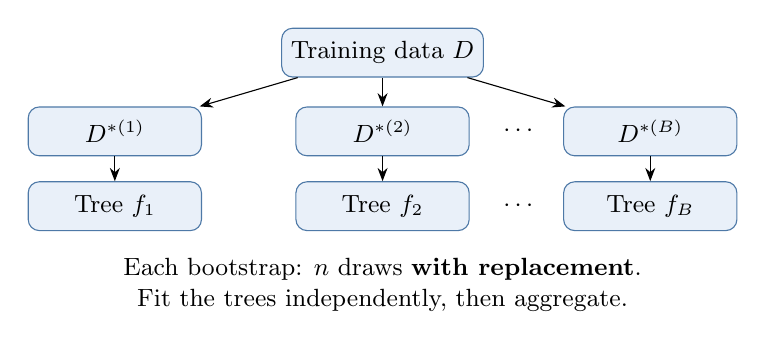
\begin{tikzpicture}[every node/.style={font=\small},box/.style={rounded corners,draw=blueplot,fill=definitionblue,minimum width=2.2cm,minimum height=.62cm,align=center}]
\node[box] (data) at (0,0) {Training data $D$};
\node[box] (d1) at (-3.4,-1.0) {$D^{*(1)}$};\node[box] (d2) at (0,-1.0) {$D^{*(2)}$};\node[box] (db) at (3.4,-1.0) {$D^{*(B)}$};
\node[box] (t1) at (-3.4,-1.95) {Tree $f_1$};\node[box] (t2) at (0,-1.95) {Tree $f_2$};\node[box] (tb) at (3.4,-1.95) {Tree $f_B$};
\foreach \a/\b in {data/d1,data/d2,data/db,d1/t1,d2/t2,db/tb}{\draw[-{Stealth}] (\a)--(\b);}
\node at (1.75,-1.0) {$\cdots$};\node at (1.75,-1.95) {$\cdots$};
\node[align=center] at (0,-2.95) {Each bootstrap: $n$ draws \textbf{with replacement}.\\Fit the trees independently, then aggregate.};
\end{tikzpicture}
\end{center}
\begin{definitionbox}Regression: $\displaystyle\bar f(x)=\frac1B\sum_{b=1}^Bf_b(x)$.\quad Classification: plurality vote among tree labels.\end{definitionbox}
\note{Source: Breiman, Bagging Predictors. Each bootstrap has n draws but repeats some rows and omits others. Trees can be fitted independently conditional on the original dataset. Classification here uses label voting, consistent with the original description; probability averaging is another common convention. A base tree need not be deliberately weak. Bagging can reduce variance for unstable learners but is not a universal improvement for every learner or problem.}
\end{frame}

\begin{frame}[t]{Why averaging can reduce variance}
\lead{Fix an input $x$. View tree predictions $f_b(x)$ as random variables.}
\begin{definitionbox}Assume $\Var(f_b(x))=v$ and $\Cov(f_b(x),f_c(x))=\rho v$ for $b\ne c$.\end{definitionbox}
\[\begin{aligned}
\Var\!\left(\frac1B\sum_{b=1}^Bf_b(x)\right)
 &=\frac1{B^2}\left[\sum_b\Var(f_b(x))+\sum_{b\ne c}\Cov(f_b(x),f_c(x))\right]\\[6pt]
\uncover<2->{&=\frac{Bv+B(B-1)\rho v}{B^2}}\\[6pt]
\uncover<2->{&=\boxed{\rho v+\frac{(1-\rho)v}{B}}.}
\end{aligned}\]
\uncover<2->{\begin{takeaway}Lower correlation makes averaging more effective.\end{takeaway}}
\note{Randomness can include the training sample and bootstrap or feature randomization. At fixed x, equal variances and equal pairwise correlations yield an exact algebraic identity. With independent bootstrap seeds conditional on a fixed dataset, predictions can be conditionally independent; shared training data induces dependence across repeated datasets. This is a schematic explanation of unconditional prediction variance, not a claim that empirical tree pairs have identical correlations. It removes neither bias nor irreducible noise and is not an MSE guarantee.}
\end{frame}

\begin{frame}[t]{Correlation limits the benefit}
\begin{columns}[T,onlytextwidth]
\column{.65\textwidth}\vspace{.25cm}\fig{foundations-correlation}
\column{.32\textwidth}\vspace{.35cm}
\begin{definitionbox}At $B=100$:
\[\begin{array}{c|c}\rho&\Var(\bar f)/v\\\hline0&0.01\\0.2&0.208\\0.8&0.802\end{array}\]
\end{definitionbox}
\small More trees reduce the second term.\par
\prompt{How can we also reduce correlation?}
\end{columns}
\note{Analytical curves plot rho+(1-rho)/B, not estimated learning curves. Nonnegative correlations are illustrative and fixed while B varies. Identical predictions have rho=1, giving no variance reduction. Random forests vary candidate features so a dominant feature does not force similar early splits in every tree. The outcome depends on data and individual-tree strength.}
\end{frame}

\input{transition-06-forests.tex}

\begin{frame}[t]{Random forests vary each split}
\lead{Bootstrap the rows; sample a fresh subset of candidate features at every node.}
\begin{columns}[T,onlytextwidth]
\column{.53\textwidth}\centering
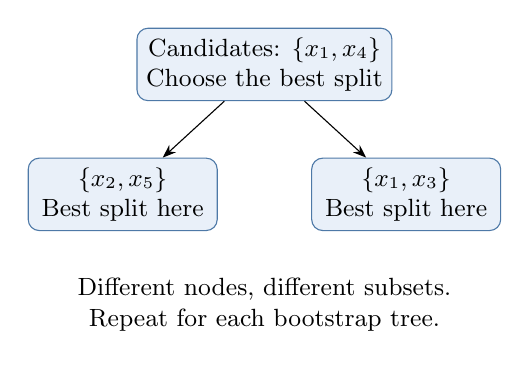
\begin{tikzpicture}[every node/.style={font=\small},box/.style={draw=blueplot,fill=definitionblue,rounded corners,align=center,minimum height=.9cm,minimum width=2.4cm}]
\node[box] (root) at (0,0) {Candidates: $\{x_1,x_4\}$\\Choose the best split};
\node[box] (l) at (-1.8,-1.65) {$\{x_2,x_5\}$\\Best split here};\node[box] (r) at (1.8,-1.65) {$\{x_1,x_3\}$\\Best split here};
\draw[-{Stealth}] (root)--(l);\draw[-{Stealth}] (root)--(r);
\node[align=center] at (0,-3.05) {Different nodes, different subsets.\\Repeat for each bootstrap tree.};
\end{tikzpicture}
\column{.43\textwidth}
\begin{definitionbox}At each node:
\begin{enumerate}\item Sample $m$ of the $d$ features.\item Search splits using these features.\item Keep the best split.\end{enumerate}
\end{definitionbox}
\small Smaller $m$ can reduce tree correlation, but may weaken each tree.\par Tune feature count and leaf complexity.
\end{columns}
\note{Source: Breiman and Cutler. Feature subsets are schematic with d=5 and m=2. A fresh subset is drawn at each node, not once per tree or forest. We describe standard bootstrap random forests; other variants exist. Use regression means and classification label votes here. Neither bagging nor forests is guaranteed never to overfit. Tree count mainly controls averaging accuracy; depth, leaf size and feature subsampling also affect the fitted predictor.}
\end{frame}

\begin{frame}[t]{Out-of-bag prediction}
\lead{For row $i$, predict using only trees whose bootstrap sample omitted row $i$.}
\begin{columns}[T,onlytextwidth]
\column{.47\textwidth}
\begin{definitionbox}A row is absent from one bootstrap with probability
\[\begin{aligned}\Pr(i\text{ omitted})&=\left(1-\frac1n\right)^n\\[4pt]&\longrightarrow e^{-1}\approx0.368.\end{aligned}\]
\end{definitionbox}
\small Evaluate each row using its own out-of-bag trees, then average the losses.
\column{.49\textwidth}\small Example: $n=5$ rows, three bootstrap samples.\vspace{.2cm}
\begin{tabular}{cll}\toprule Tree & Sampled row IDs & Omitted IDs\\\midrule
$1$ & $1,1,2,4,5$ & $\mathbf{3}$\\$2$ & $2,3,3,4,4$ & $1,5$\\$3$ & $1,2,2,3,5$ & $4$\\\bottomrule\end{tabular}
\vspace{.3cm}
\begin{takeaway}Row $3$ is evaluated with tree $1$ only in this tiny example.\end{takeaway}
\end{columns}
\note{The exact exclusion probability is (1-1/n)^n; 0.368 is its large-n limit. For regression average a row's OOB trees, and for classification vote. With too few trees some rows have no OOB prediction. OOB assessment is useful for bagging and bootstrap forests. Repeated tuning against OOB scores can bias selection; final assessment needs an appropriate held-out protocol, especially for dependent or shifted data.}
\end{frame}

\begin{frame}[t]{Two ways to build a stronger predictor}
\begin{columns}[T,onlytextwidth]
\column{.48\textwidth}
\begin{definitionbox}\textbf{Boosting}\par Fit the next learner to improve the current ensemble.
\[F_0\;\longrightarrow\;F_1\;\longrightarrow\;\cdots\;\longrightarrow\;F_M\]
\[F_m=F_{m-1}+\alpha_m h_m.\]
\end{definitionbox}
\small AdaBoost: reweight difficult examples.\par
Gradient boosting: fit negative gradients.\par
Often use small, restricted base learners.
\column{.48\textwidth}
\begin{definitionbox}\textbf{Bagging / random forests}\par Fit diverse trees independently; average or vote.
\[D\;\longrightarrow\;\begin{cases}f_1\\f_2\\\vdots\\f_B\end{cases}\;\longrightarrow\;\bar f\]
\end{definitionbox}
\small Stabilize variable predictions.\par
Often use deep, individually flexible trees.\par
Forests add random feature subsets.
\end{columns}
\begin{takeaway}Both combine models. Their training mechanisms and guarantees differ.\end{takeaway}
\note{This compares methods already covered rather than announcing AdaBoost. Boosting stages depend on previous stages; bagged trees train independently across trees conditional on the original dataset. Computations within one boosting stage can still be parallel. The AdaBoost training-error bound requires a weighted error below one half at each relevant round; averaging arbitrary models alone has no analogous weak-learning guarantee. Bagging often uses deep trees with high variance, not necessarily weak learners. Variance reduction, bias reduction, and predictive accuracy are not exclusive to one family: state the mechanisms rather than a rigid bias-versus-variance taxonomy. The next case shows randomized forests in Kinect body tracking.}
\end{frame}

	\SectionSlide{Bagging: Learning by Averaging}{}
	% Bagging: a short, standalone section for the existing lecture.
% Include inside the document body with: % Bagging: a short, standalone section for the existing lecture.
% Include inside the document body with: % Bagging: a short, standalone section for the existing lecture.
% Include inside the document body with: \input{bagging.tex}
% Uses the existing theme.tex (Beamer, TikZ, PGFPlots, definitionbox, takeaway).
% No external figures, data files, or additional project macros are required.
% Seven logical frames; two frames use a second reveal. Presenter notes included.


\begin{frame}[t]{Bootstrap Aggregation}
	\lead{Training set $D=\{(x_i,y_i)\}_{i=1}^{n}$. Choose a base learner and a model count $B$.}
	\begin{center}
		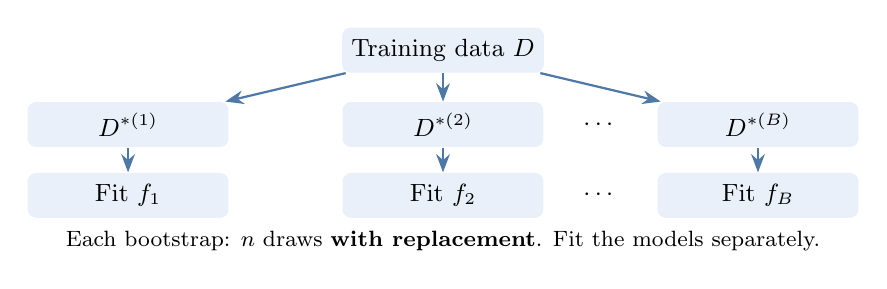
\begin{tikzpicture}[x=1cm,y=.9cm,>=Stealth,
			every node/.style={font=\small},
			stage/.style={rounded corners=3pt,draw=none,fill=definitionblue,
				minimum width=2.55cm,minimum height=.57cm,align=center}]
			\node[stage] (data) at (0,0) {Training data $D$};
			\node[stage] (d1) at (-4,-1.05) {$D^{*(1)}$};
			\node[stage] (d2) at (0,-1.05) {$D^{*(2)}$};
			\node[stage] (db) at (4,-1.05) {$D^{*(B)}$};
			\node[stage] (f1) at (-4,-2.05) {Fit $f_1$};
			\node[stage] (f2) at (0,-2.05) {Fit $f_2$};
			\node[stage] (fb) at (4,-2.05) {Fit $f_B$};
			\foreach \a/\b in {data/d1,data/d2,data/db,d1/f1,d2/f2,db/fb}
			{\draw[->,thick,blueplot] (\a)--(\b);}
			\node at (2,-1.05) {$\cdots$};
			\node at (2,-2.05) {$\cdots$};
			\node[font=\footnotesize] at (0,-2.7)
			{Each bootstrap: $n$ draws \textbf{with replacement}. Fit the models separately.};
		\end{tikzpicture}
	\end{center}
	\uncover<2->{
		\begin{definitionbox}
			\textbf{Regression:}\quad $\displaystyle \widehat f_{\mathrm{bag}}(x)=\frac1B\sum_{b=1}^{B}f_b(x)$.
			\par\vspace{.09cm}
			\textbf{Classification:}\quad take the most frequent predicted class.
	\end{definitionbox}}
	\vfill
	{\scriptsize\href{https://www.stat.berkeley.edu/~breiman/bagging.pdf}{Breiman, \emph{Bagging Predictors}, Section 1.}\par}
	\note{Use the same learning procedure on every bootstrap sample; fitted parameters differ because the sampled observations differ. The draws are uniform over the original training rows and independent with replacement. Each sample contains n draws, not necessarily n distinct observations. There is no residual target or error-dependent reweighting between fitted models. With independent sampling and training seeds, fits can be computed independently conditional on D and can be parallelized. Regression averages numerical predictions. Classification can use a plurality vote with a fixed tie rule; averaging class-probability vectors before taking the largest component is another common convention. Bagging does not generate new independent information about the population.}
\end{frame}




\begin{frame}[t]{Bagging for Movie Ratings}
	\lead{Predict a user's rating for a movie they have not rated.}
	\begin{columns}[T,onlytextwidth]
		\column{.48\textwidth}
		\begin{definitionbox}
			\textbf{Base model: matrix factorization}\par
			User vector $p_u$; movie vector $q_i$:
			\[
			\widehat r_{ui}=p_u^{\mathsf T}q_i.
			\]
		\end{definitionbox}
		\vspace{.08cm}
		\small Bootstrap the $(\text{user},\text{movie},\text{rating})$ records.\par
		Fit one scoring model per sample.\par
		Average the predicted ratings:
		\[
		\widehat r_{ui}^{\mathrm{bag}}=\frac1B\sum_{b=1}^{B}\widehat r_{ui}^{(b)}.
		\]
		\column{.48\textwidth}
		\uncover<2->{
			\begin{definitionbox}
				\textbf{MovieLens 100K: reported RMSE}\par
				\vspace{.18cm}
				\begin{tabular}{@{}lr@{}}
					Single ISMF model & $0.9434$\\[9pt]
					Bagging, $B=50$ & $\mathbf{0.9173}$
				\end{tabular}
			\end{definitionbox}
			\vspace{.16cm}
			\begin{takeaway}
				One algorithm, many resampled fits.\par
				Lower RMSE in this experiment.
			\end{takeaway}
			\vspace{.16cm}
			\small Offline result on real rating data.
		}
	\end{columns}
	\vfill
	{\scriptsize\href{https://arxiv.org/pdf/1211.2891}{Bar et al. (2012), Section 4.1 and Table 1: MovieLens 100K results.}\par}
	\note{This paper studies several ensemble methods; use only its bagging results here. Section 4.1 explicitly samples rating records with replacement, trains one collaborative-filtering model per sample, and averages predictions. The displayed matrix-factorization expression explains the basic scoring mechanism; ISMF is the specific matrix-factorization baseline used for the quoted table values. Learners must account for repeated ratings or equivalent multiplicity weights. The 50-model ISMF bagging value and single-model value come from the MovieLens 100K comparison in Table 1; do not replace ISMF with an arbitrary modern matrix-factorization baseline. The paper reports the best tested configuration of each method, evaluated over five random 80:20 splits. Average model predictions, not the separately learned latent vectors, whose coordinates need not align. This is historical offline research evidence, not a Netflix production-deployment claim. Rating RMSE alone does not establish better ranking, engagement, or revenue. No new factorization derivation is required for this application slide.}
\end{frame}

\begin{frame}[t]{When and How to Use Bagging}
	\begin{columns}[T,onlytextwidth]
		\column{.47\textwidth}
		\begin{definitionbox}
			\textbf{Look for an unstable base learner}\par
			Small changes to the training data can produce noticeably different predictions.
		\end{definitionbox}
		\vspace{.12cm}
		\small Examples: flexible trees, neural networks, or regression with variable selection.\par
		\vspace{.20cm}
		\textbf{Account for the cost}\par
		Store and evaluate $B$ fitted models.\par
		Separate fits can be trained in parallel.
		\column{.49\textwidth}
		\begin{definitionbox}
			\textbf{A practical workflow}
			\begin{enumerate}
				\setlength{\itemsep}{.14cm}
				\item Reserve evaluation data before fitting.
				\item Bootstrap the training portion only.
				\item Tune using validation error.
				\item Assess the selected ensemble on held-out test data.
			\end{enumerate}
		\end{definitionbox}
	\end{columns}
\end{frame}



% Uses the existing theme.tex (Beamer, TikZ, PGFPlots, definitionbox, takeaway).
% No external figures, data files, or additional project macros are required.
% Seven logical frames; two frames use a second reveal. Presenter notes included.


\begin{frame}[t]{Bootstrap Aggregation}
	\lead{Training set $D=\{(x_i,y_i)\}_{i=1}^{n}$. Choose a base learner and a model count $B$.}
	\begin{center}
		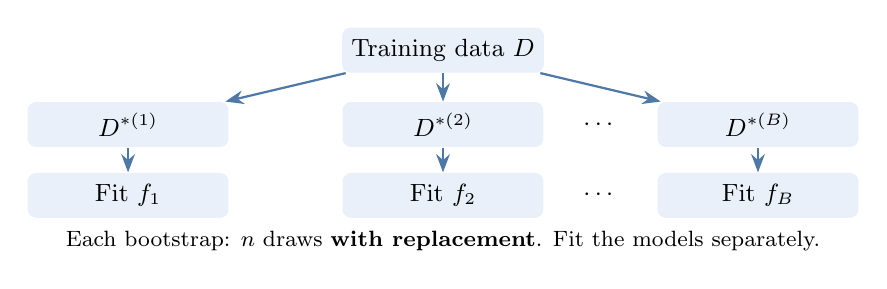
\begin{tikzpicture}[x=1cm,y=.9cm,>=Stealth,
			every node/.style={font=\small},
			stage/.style={rounded corners=3pt,draw=none,fill=definitionblue,
				minimum width=2.55cm,minimum height=.57cm,align=center}]
			\node[stage] (data) at (0,0) {Training data $D$};
			\node[stage] (d1) at (-4,-1.05) {$D^{*(1)}$};
			\node[stage] (d2) at (0,-1.05) {$D^{*(2)}$};
			\node[stage] (db) at (4,-1.05) {$D^{*(B)}$};
			\node[stage] (f1) at (-4,-2.05) {Fit $f_1$};
			\node[stage] (f2) at (0,-2.05) {Fit $f_2$};
			\node[stage] (fb) at (4,-2.05) {Fit $f_B$};
			\foreach \a/\b in {data/d1,data/d2,data/db,d1/f1,d2/f2,db/fb}
			{\draw[->,thick,blueplot] (\a)--(\b);}
			\node at (2,-1.05) {$\cdots$};
			\node at (2,-2.05) {$\cdots$};
			\node[font=\footnotesize] at (0,-2.7)
			{Each bootstrap: $n$ draws \textbf{with replacement}. Fit the models separately.};
		\end{tikzpicture}
	\end{center}
	\uncover<2->{
		\begin{definitionbox}
			\textbf{Regression:}\quad $\displaystyle \widehat f_{\mathrm{bag}}(x)=\frac1B\sum_{b=1}^{B}f_b(x)$.
			\par\vspace{.09cm}
			\textbf{Classification:}\quad take the most frequent predicted class.
	\end{definitionbox}}
	\vfill
	{\scriptsize\href{https://www.stat.berkeley.edu/~breiman/bagging.pdf}{Breiman, \emph{Bagging Predictors}, Section 1.}\par}
	\note{Use the same learning procedure on every bootstrap sample; fitted parameters differ because the sampled observations differ. The draws are uniform over the original training rows and independent with replacement. Each sample contains n draws, not necessarily n distinct observations. There is no residual target or error-dependent reweighting between fitted models. With independent sampling and training seeds, fits can be computed independently conditional on D and can be parallelized. Regression averages numerical predictions. Classification can use a plurality vote with a fixed tie rule; averaging class-probability vectors before taking the largest component is another common convention. Bagging does not generate new independent information about the population.}
\end{frame}




\begin{frame}[t]{Bagging for Movie Ratings}
	\lead{Predict a user's rating for a movie they have not rated.}
	\begin{columns}[T,onlytextwidth]
		\column{.48\textwidth}
		\begin{definitionbox}
			\textbf{Base model: matrix factorization}\par
			User vector $p_u$; movie vector $q_i$:
			\[
			\widehat r_{ui}=p_u^{\mathsf T}q_i.
			\]
		\end{definitionbox}
		\vspace{.08cm}
		\small Bootstrap the $(\text{user},\text{movie},\text{rating})$ records.\par
		Fit one scoring model per sample.\par
		Average the predicted ratings:
		\[
		\widehat r_{ui}^{\mathrm{bag}}=\frac1B\sum_{b=1}^{B}\widehat r_{ui}^{(b)}.
		\]
		\column{.48\textwidth}
		\uncover<2->{
			\begin{definitionbox}
				\textbf{MovieLens 100K: reported RMSE}\par
				\vspace{.18cm}
				\begin{tabular}{@{}lr@{}}
					Single ISMF model & $0.9434$\\[9pt]
					Bagging, $B=50$ & $\mathbf{0.9173}$
				\end{tabular}
			\end{definitionbox}
			\vspace{.16cm}
			\begin{takeaway}
				One algorithm, many resampled fits.\par
				Lower RMSE in this experiment.
			\end{takeaway}
			\vspace{.16cm}
			\small Offline result on real rating data.
		}
	\end{columns}
	\vfill
	{\scriptsize\href{https://arxiv.org/pdf/1211.2891}{Bar et al. (2012), Section 4.1 and Table 1: MovieLens 100K results.}\par}
	\note{This paper studies several ensemble methods; use only its bagging results here. Section 4.1 explicitly samples rating records with replacement, trains one collaborative-filtering model per sample, and averages predictions. The displayed matrix-factorization expression explains the basic scoring mechanism; ISMF is the specific matrix-factorization baseline used for the quoted table values. Learners must account for repeated ratings or equivalent multiplicity weights. The 50-model ISMF bagging value and single-model value come from the MovieLens 100K comparison in Table 1; do not replace ISMF with an arbitrary modern matrix-factorization baseline. The paper reports the best tested configuration of each method, evaluated over five random 80:20 splits. Average model predictions, not the separately learned latent vectors, whose coordinates need not align. This is historical offline research evidence, not a Netflix production-deployment claim. Rating RMSE alone does not establish better ranking, engagement, or revenue. No new factorization derivation is required for this application slide.}
\end{frame}

\begin{frame}[t]{When and How to Use Bagging}
	\begin{columns}[T,onlytextwidth]
		\column{.47\textwidth}
		\begin{definitionbox}
			\textbf{Look for an unstable base learner}\par
			Small changes to the training data can produce noticeably different predictions.
		\end{definitionbox}
		\vspace{.12cm}
		\small Examples: flexible trees, neural networks, or regression with variable selection.\par
		\vspace{.20cm}
		\textbf{Account for the cost}\par
		Store and evaluate $B$ fitted models.\par
		Separate fits can be trained in parallel.
		\column{.49\textwidth}
		\begin{definitionbox}
			\textbf{A practical workflow}
			\begin{enumerate}
				\setlength{\itemsep}{.14cm}
				\item Reserve evaluation data before fitting.
				\item Bootstrap the training portion only.
				\item Tune using validation error.
				\item Assess the selected ensemble on held-out test data.
			\end{enumerate}
		\end{definitionbox}
	\end{columns}
\end{frame}



% Uses the existing theme.tex (Beamer, TikZ, PGFPlots, definitionbox, takeaway).
% No external figures, data files, or additional project macros are required.
% Seven logical frames; two frames use a second reveal. Presenter notes included.


\begin{frame}[t]{Bootstrap Aggregation}
	\lead{Training set $D=\{(x_i,y_i)\}_{i=1}^{n}$. Choose a base learner and a model count $B$.}
	\begin{center}
		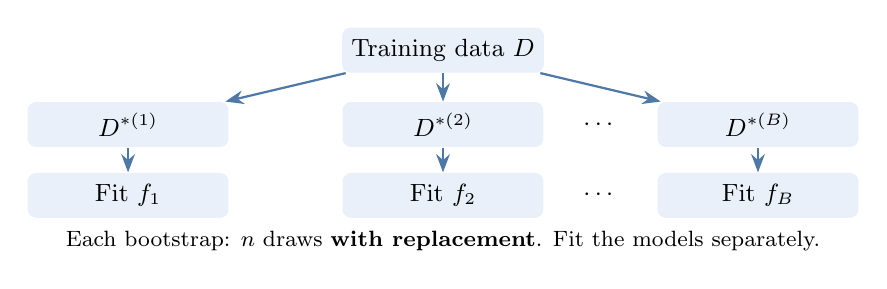
\begin{tikzpicture}[x=1cm,y=.9cm,>=Stealth,
			every node/.style={font=\small},
			stage/.style={rounded corners=3pt,draw=none,fill=definitionblue,
				minimum width=2.55cm,minimum height=.57cm,align=center}]
			\node[stage] (data) at (0,0) {Training data $D$};
			\node[stage] (d1) at (-4,-1.05) {$D^{*(1)}$};
			\node[stage] (d2) at (0,-1.05) {$D^{*(2)}$};
			\node[stage] (db) at (4,-1.05) {$D^{*(B)}$};
			\node[stage] (f1) at (-4,-2.05) {Fit $f_1$};
			\node[stage] (f2) at (0,-2.05) {Fit $f_2$};
			\node[stage] (fb) at (4,-2.05) {Fit $f_B$};
			\foreach \a/\b in {data/d1,data/d2,data/db,d1/f1,d2/f2,db/fb}
			{\draw[->,thick,blueplot] (\a)--(\b);}
			\node at (2,-1.05) {$\cdots$};
			\node at (2,-2.05) {$\cdots$};
			\node[font=\footnotesize] at (0,-2.7)
			{Each bootstrap: $n$ draws \textbf{with replacement}. Fit the models separately.};
		\end{tikzpicture}
	\end{center}
	\uncover<2->{
		\begin{definitionbox}
			\textbf{Regression:}\quad $\displaystyle \widehat f_{\mathrm{bag}}(x)=\frac1B\sum_{b=1}^{B}f_b(x)$.
			\par\vspace{.09cm}
			\textbf{Classification:}\quad take the most frequent predicted class.
	\end{definitionbox}}
	\vfill
	{\scriptsize\href{https://www.stat.berkeley.edu/~breiman/bagging.pdf}{Breiman, \emph{Bagging Predictors}, Section 1.}\par}
	\note{Use the same learning procedure on every bootstrap sample; fitted parameters differ because the sampled observations differ. The draws are uniform over the original training rows and independent with replacement. Each sample contains n draws, not necessarily n distinct observations. There is no residual target or error-dependent reweighting between fitted models. With independent sampling and training seeds, fits can be computed independently conditional on D and can be parallelized. Regression averages numerical predictions. Classification can use a plurality vote with a fixed tie rule; averaging class-probability vectors before taking the largest component is another common convention. Bagging does not generate new independent information about the population.}
\end{frame}




\begin{frame}[t]{Bagging for Movie Ratings}
	\lead{Predict a user's rating for a movie they have not rated.}
	\begin{columns}[T,onlytextwidth]
		\column{.48\textwidth}
		\begin{definitionbox}
			\textbf{Base model: matrix factorization}\par
			User vector $p_u$; movie vector $q_i$:
			\[
			\widehat r_{ui}=p_u^{\mathsf T}q_i.
			\]
		\end{definitionbox}
		\vspace{.08cm}
		\small Bootstrap the $(\text{user},\text{movie},\text{rating})$ records.\par
		Fit one scoring model per sample.\par
		Average the predicted ratings:
		\[
		\widehat r_{ui}^{\mathrm{bag}}=\frac1B\sum_{b=1}^{B}\widehat r_{ui}^{(b)}.
		\]
		\column{.48\textwidth}
		\uncover<2->{
			\begin{definitionbox}
				\textbf{MovieLens 100K: reported RMSE}\par
				\vspace{.18cm}
				\begin{tabular}{@{}lr@{}}
					Single ISMF model & $0.9434$\\[9pt]
					Bagging, $B=50$ & $\mathbf{0.9173}$
				\end{tabular}
			\end{definitionbox}
			\vspace{.16cm}
			\begin{takeaway}
				One algorithm, many resampled fits.\par
				Lower RMSE in this experiment.
			\end{takeaway}
			\vspace{.16cm}
			\small Offline result on real rating data.
		}
	\end{columns}
	\vfill
	{\scriptsize\href{https://arxiv.org/pdf/1211.2891}{Bar et al. (2012), Section 4.1 and Table 1: MovieLens 100K results.}\par}
	\note{This paper studies several ensemble methods; use only its bagging results here. Section 4.1 explicitly samples rating records with replacement, trains one collaborative-filtering model per sample, and averages predictions. The displayed matrix-factorization expression explains the basic scoring mechanism; ISMF is the specific matrix-factorization baseline used for the quoted table values. Learners must account for repeated ratings or equivalent multiplicity weights. The 50-model ISMF bagging value and single-model value come from the MovieLens 100K comparison in Table 1; do not replace ISMF with an arbitrary modern matrix-factorization baseline. The paper reports the best tested configuration of each method, evaluated over five random 80:20 splits. Average model predictions, not the separately learned latent vectors, whose coordinates need not align. This is historical offline research evidence, not a Netflix production-deployment claim. Rating RMSE alone does not establish better ranking, engagement, or revenue. No new factorization derivation is required for this application slide.}
\end{frame}

\begin{frame}[t]{When and How to Use Bagging}
	\begin{columns}[T,onlytextwidth]
		\column{.47\textwidth}
		\begin{definitionbox}
			\textbf{Look for an unstable base learner}\par
			Small changes to the training data can produce noticeably different predictions.
		\end{definitionbox}
		\vspace{.12cm}
		\small Examples: flexible trees, neural networks, or regression with variable selection.\par
		\vspace{.20cm}
		\textbf{Account for the cost}\par
		Store and evaluate $B$ fitted models.\par
		Separate fits can be trained in parallel.
		\column{.49\textwidth}
		\begin{definitionbox}
			\textbf{A practical workflow}
			\begin{enumerate}
				\setlength{\itemsep}{.14cm}
				\item Reserve evaluation data before fitting.
				\item Bootstrap the training portion only.
				\item Tune using validation error.
				\item Assess the selected ensemble on held-out test data.
			\end{enumerate}
		\end{definitionbox}
	\end{columns}
\end{frame}



%% Two frames / three physical pages. Original explanatory schematics.
\begin{frame}[t]{Kinect: trees recognize body parts}
\lead{Real deployment: body-pose estimation for controller-free games.}
\begin{center}\fig{case-kinect-pipeline}\end{center}
\pause
\begin{takeaway}Turn a pose-estimation problem into many \textbf{body-part classification} problems.\end{takeaway}
\vspace{.12cm}
{\scriptsize\href{https://www.microsoft.com/en-us/research/wp-content/uploads/2016/02/BodyPartRecognition.pdf}{Shotton et al., CVPR 2011, Sections 1 and 3.}\par}
\note{The paper identifies this method as a core Kinect component. The illustration explains the pipeline; it is not a captured camera frame or a model output. First describe the practical need to recover pose after tracking fails, then reveal the classification reformulation.}
\end{frame}

\begin{frame}[t]{From tree probabilities to joint positions}
\lead{A randomized decision forest classifies each depth-image pixel.}
\begin{columns}[T,onlytextwidth]
\column{.56\textwidth}\centering\fig{case-kinect-forest}
\column{.40\textwidth}
\begin{definitionbox}\raggedright
\textbf{Published configuration}\par
31 body-part labels\par
3 trees; depth 20
\end{definitionbox}
\begin{takeaway}\raggedright
\textbf{Reported algorithm speed}\par
Under 5 ms/frame\par
Xbox 360 GPU\par
\smallskip
Camera input: 30 frames/s
\end{takeaway}
\vspace{.14cm}{\small Crossed arms and unseen poses can still cause errors.}
\end{columns}
\vspace{.08cm}
{\scriptsize\href{https://www.microsoft.com/en-us/research/wp-content/uploads/2016/02/BodyPartRecognition.pdf}{Shotton et al. (2011), Sections 1, 2.1, 3.3--3.4, and 4.}\par}
\note{Trees use separate synthetic-image sets and randomized candidate splits, not textbook bootstrap bagging. Leaf probabilities are averaged; spatial mode finding produces joint proposals. The speed is the paper's optimized algorithm, not the complete Kinect system. These historical results do not establish present-day performance.}
\end{frame}

%\begin{frame}[t]{How do the models work together?}
\small\renewcommand{\arraystretch}{1.35}
\begin{tabularx}{\textwidth}{@{}p{.20\textwidth}YY@{}}
\toprule
\textbf{Method}&\textbf{How the next model is fitted}&\textbf{How predictions combine}\\\midrule
AdaBoost&Fit a classifier under updated observation weights.&Weighted vote through $\sum_m\alpha_m h_m(x)$.\\[5pt]
Gradient boosting&Fit a learner to a loss-gradient target.&Add corrections to scores or responses.\\[5pt]
Bagging / RF&Resampled observations; RF also samples candidate features.&Average values or aggregate class predictions.\\\bottomrule
\end{tabularx}
\vspace{.15cm}\begin{takeaway}The loss, the base learner, and the way models are combined define the method.\end{takeaway}
\note{Avoid equating bagging exclusively with variance reduction or boosting exclusively with bias reduction; these are intuitions, not universal decompositions. The variance formula earlier concerned a fixed input and repeated training samples. AdaBoost's training-error guarantee does not guarantee test performance. For binary gradient boosting, sum scores then apply sigmoid once. For random forests, averaging per-tree probabilities and majority voting need not make identical decisions.}
\end{frame}

\begin{frame}[t]{References and further reading}
\small
\begin{itemize}\setlength{\itemsep}{.15cm}
\item Freund and Schapire (1997). \href{https://doi.org/10.1006/jcss.1997.1504}{\textit{A Decision-Theoretic Generalization of On-Line Learning and an Application to Boosting}.}
\item Friedman (2001). \href{https://doi.org/10.1214/aos/1013203451}{\textit{Greedy Function Approximation: A Gradient Boosting Machine}.}
\item Breiman (1996). \href{https://statistics.berkeley.edu/tech-reports/421}{\textit{Bagging Predictors}.}
\item Breiman (2001). \href{https://www.stat.berkeley.edu/~breiman/randomforest2001.pdf}{\textit{Random Forests}.}
\end{itemize}
\note{Clickable primary references. Supporting sections and derivation conventions appear in module source ledgers. Figures distinguish constructed demonstrations, sourced measurements, and explanatory diagrams. The AdaBoost module also cites Schapire2003 for exponential loss and the training-error bound. Numerical scripts validate displayed calculations.}
\end{frame}

%\begin{frame}[t]{Sources for the application cases}
\small
\begin{itemize}\setlength{\itemsep}{.24cm}
\item Amatriain and Basilico (2012). \href{https://netflixtechblog.com/netflix-recommendations-beyond-the-5-stars-part-1-55838468f429}{\textit{Netflix Recommendations: Beyond the 5 Stars (Part 1)}. Netflix Technology Blog.}
\item He et al. (2014). \href{https://quinonero.net/Publications/predicting-clicks-facebook.pdf}{\textit{Practical Lessons from Predicting Clicks on Ads at Facebook}.}
\item Ben Taieb and Hyndman (2014). \href{https://robjhyndman.com/papers/kaggle-competition.pdf}{\textit{A Gradient Boosting Approach to the Kaggle Load Forecasting Competition}.}
\item Shotton et al. (2011). \href{https://www.microsoft.com/en-us/research/wp-content/uploads/2016/02/BodyPartRecognition.pdf}{\textit{Real-Time Human Pose Recognition in Parts from Single Depth Images}.}
\end{itemize}
\note{These historical sources document the applications. Case-specific source ledgers identify sections and metric conventions. Published results were checked against the original papers; no source result is presented as a new experiment.}
\end{frame}

\end{document}
